\section{Module: aipy.miriad}
\label{sec:intro}

This module forms provides access to Miriad UV files from Python.  Miriad
(Multichannel Image Reconstruction Image Analysis and Display) is
a primarily Fortran package (with some C for file IO) for reducing
interferometric data.  It was commissioned in 1988 and is still in active
use, particularly at the Australia Telescope National Facility (ATNF).  The 
uv file format defined by Miriad is quite flexible, and is capable of storing
many different kinds of observations compactly.  For the sake of simplicity,
this Python wrapper only supports the multi-channel spectrum mode (corr,
not wcorr, for you Miriad mavens).  

The UV class in aipy.miriad attempts to construct a pythonic interface to uv
files that abstracts away some of the complex details of Miriad file handling.
Nonetheless, understanding of the basic model of a uv file can only help the
programmer, so we'll provide a brief summary in the following section.  Further
information is available in the Miriad User Guide available at {\it
http://www.atnf.csiro.au/computing/software/miriad/}.  After gaining an
understanding of the file format, we will demonstrate the basic functionality
of the UV class.  Finally, there will be a more detailed ``under the hood''
look at the UV class for those who may need to extend its functionality.

\subsection{Miriad's UV File Format}

\subsubsection{Header Items}
UV datasets are directories containing files.  These files each contain
various numbers of header items, and a header item can represent anything from
a single integer to the entire correlation data.  Small header items are
grouped into a file called ``header''.  Large header items (like the
correlation data) have files of their own.  Header items are static;
their values do not change as you read through the data in a file.

\subsubsection{Correlation Data and Variables}
The most important header item is the correlation data stored
in ``visdata''.  This header is not accessed like others--instead of
reading the entire data, you step through it spectrum by spectrum.  As you do
so, various variables (which are distinct from header items) become accessible
to provide you with information about the spectrum you just read.  A list of
all variables in the file, and their types, are in the header item ``vartable''.
Miriad correlation data is a {\bf stream}.  Variables are set at the beginning,
and thereafter only the changes from previous values are stored.  Thus, to
know the value of ``pol'' for a given spectrum, you will have to know the
value of the last relevant tag that was inserted in the datastream.
UV files are not random-access, much like a cassette tape; you can
``fast-forward'', but you cannot ``skip''.

Two variables you will be accessing regularly require a little more
explanation.  Miriad convention is to reference a baseline from antenna i to
antenna j (counting from 1) as: $(i << 8) | j$.  Steps have been taken to
conseal this in the wrapper, which instead references a baseline as
zero-indexed tuple $(i^\prime, j^\prime)$, where $i^\prime = i-1$ and $j^\prime
= j-1$.  Though they shouldn't be necessary, conversion functions bl2ij() and
ij2bl() are provided in aipy.miriad, where ``bl'' is the Miriad code, and
``ij'' is a zero-indexed tuple.  The second variable which warrants discussion 
is polarization (``pol'').  Miriad uses an integer code to store polarization.  
Dictionary converters for integer codes and more informative string 
representations are provided as aipy.miriad.pol2str and aipy.miriad.str2pol, 
but no steps have been taken to automatically convert these codes in the
wrapper.

\subsubsection{The Preamble}
Some variables will likely change nearly every spectrum.  Among these are
the projected uvw coordinates of a baseline, the time the data were captured,
and the baseline index.  Since you'll need these with every spectrum you read,
Miriad provides them to you along with the data in the form of a ``preamble''.
Thus, when you read a spectrum, you get 2 things: a preamble and a data.
Although Miriad gives some limited ability to select which variables are
included in the preamble, the Python wrapper statically sets it to be
(uvw, time, baseline) to avoid complexity.

\subsubsection{Flags}
Not all of your data may be valid.  Miriad provides boolean flags along with 
your data to keep you informed.  Although these flags are natively stored
oppositely, this wrapper provides them as part of the mask in a Numpy masked
array where the convention is that 0 represents valid data, and 1 represents
masked data.  This difference in convention is consealed from the user,
and is only noted here for those who have experience using Miriad natively.

\subsection{Class: UV}

A high-level interface to a Miriad UV file is available through the 
UV class in aipy.miriad.  We'll dive right in to reading a file, but first,
so that we're working on the same UV file, run the following from bash (1 MB
download):

\begin{verbatim}
$ wget http://setiathome.berkeley.edu/~aparsons/aipy/test.uv.tar.bz2
$ compress_uv.py -x test.uv.tar.bz2
\end{verbatim}

\subsubsection{Reading an Existing File}

You should now have a test.uv file in your current directory.  Try the
following from Python:

\begin{verbatim}
>>> import aipy
>>> uv = aipy.miriad.UV('test.uv')
>>> print uv.items()
['vartable', 'obstype', 'history']
>>> print uv['history']
C2M (Python): Version=0.1.1.Fixed bandpass inversion & ordering, and pol 
label.APPLY_BP: version=0.0.1, corr type = combXRFI: version 0.0.2XTALK2: 
version 0.0.1 Miniaturized...
>>> print uv.vars()
['latitud', 'npol', 'nspect', 'obsdec', 'vsource', 'ischan', 'operator', 
'nants', 'baseline', 'sfreq', 'inttime', 'source', 'epoch', 'version', 
'ra', 'restfreq', 'nschan', 'sdf', 'corr', 'freq', 'longitu', 'nchan', 
'tscale', 'antpos', 'telescop', 'pol', 'coord', 'veldop', 'lst', 'time', 
'dec', 'obsra']
>>> print uv['nchan']
64
>>> print uv['antpos']
[  -8.48  205.47  187.1  -262.7   455.28  319.53 -352.95 -219.07    9.82
 -251.71 -232.59  318.7 ]
\end{verbatim}

First, we made an instance of a UV file (which defaulted to read an ``old''
file).  We could then ask for a list of (header) items.  Each of these header
items can then be accessed just as if uv were a dictionary holding them.  The
details of data types are taken care of automagically; strings return as Python
strings, shorts and ints return as Python integers, floats and doubles return
as Python floats.  Similarly, we can ask for a list of variables (vars), and
these are accessible as if uv were a dictionary.  As you can see, when we are
reading, there's no real need to differentiate between a header item and a
variable, and so both are accessible via the same interface.  When we access
``nchan'', which has a single value, we get that value.  When we access
``antpos'', which has multiple values, we get an array of the values.
One word of caution: don't access the ``corr'' variable.  It is evil, and
I don't know why Miriad makes it available.  Let's continue:

\begin{verbatim}
>>> preamble, data = uv.read()
>>> print preamble
(array([ 0.,  0.,  0.]), 2454302.8700115741, (0, 0))
>>> print data
[(3.55898427963+0j) (5.16037225723+0j) (7.65382957458+0j)
 (11.5349502563+0j) (17.6214637756+0j) (26.8085384369+0j)
 (40.0749702454+0j) (56.860118866+0j) (74.8811569214+0j) (89.6064910889+0j)
 (98.601524353+0j) (101.491455078+0j) (100.617973328+0j) (98.0315933228+0j)
 (95.0735092163+0j) (92.583152771+0j) (90.0556259155+0j) (88.2838745117+0j)
 (86.3324737549+0j) (84.3934631348+0j) (82.3522338867+0j) --
 (77.4334640503+0j) (74.7851333618+0j) (71.8084716797+0j)
 (68.7729568481+0j) (65.6971817017+0j) (62.5315704346+0j) (59.719078064+0j)
 (56.9530410767+0j) (54.4193191528+0j) (52.1953392029+0j)
 (50.2718162537+0j) (48.5867958069+0j) (47.1000137329+0j)
 (45.9260749817+0j) (44.9503746033+0j) (44.1512298584+0j) (43.609172821+0j)
 (43.2684516907+0j) (43.1135787964+0j) (42.8874664307+0j)
 (42.9587059021+0j) (43.0020713806+0j) (43.1228713989+0j)
 (43.1600418091+0j) (43.1321640015+0j) (43.1135787964+0j)
 (43.0020713806+0j) (42.726398468+0j) (42.5312576294+0j) (42.1409759521+0j)
 (41.6794548035+0j) (41.0073051453+0j) (40.369228363+0j) (39.5948638916+0j)
 (38.8019142151+0j) (38.0523262024+0j) (37.1168937683+0j)
 (36.1814575195+0j) (35.2924880981+0j) (34.3105926514+0j)
 (33.4278144836+0j) (32.3839683533+0j)]
>>> print uv['pol'], aipy.miriad.pol2str[uv['pol']]
-6 yy
>>> preamble, data = uv.read()
>>> print preamble
(array([-538.6,  298.79613781, -674.73816035]), 2454302.8700115741, (1, 3))
>>> print uv['time']
2454302.8700115741
\end{verbatim}

We read a preamble/data pair.  The preamble contained (uvw, time, (i,j)), and
the data was a masked, complex Numpy array.  Note that one of the entries was
masked (see the ``--''), and did not print.  If you count, there are 64
entries, just like ``nchan'' suggested.  Note also that this was an
autocorrelation (0,0), so the data has no complex component, and the uvw
corrdinates are 0.  Next, we showed how to access and convert the polarization
codes.  Following another read(), we find that we have a new preamble for
a different baseline, but for the same time.  Finally, we show that there
is nothing special about the preamble--we can access ``time'' without it if we
want to.  It's just for convenience.  Now for some more advanced stuff:

\begin{verbatim}
>>> uv.rewind()
>>> uv.select('antennae', 0, 1, include=True)
>>> for preamble, data in uv.all():
...     uvw, t, (i,j) = preamble
...     print i, j, t
...
0 1 2454302.87001
0 1 2454302.87009
0 1 2454302.87017
0 1 2454302.87025
[snip]
0 1 2454302.91135
0 1 2454302.91144
0 1 2454302.91152
0 1 2454302.9116
\end{verbatim}

First, we rewind the uv file so that we can start from the beginning again.
Next, we demonstrate a usage of select(), which allows you to choose which data
you receive via read().  In this case, we've selected to only include data
which involve antennae 0 and 1 together.  We set up a loop over all the
data in uv, split up the preamble into its components, and print the antennae
in the baseline and the time of integration.  Note that $(i,j) == (0,1)$, 
thanks to select(), and we step through all the integrations in the file.
Inside the loop, you can access variables as they change.  That's pretty much
all there is to it!

\subsubsection{Initializing and Piping From Another UV}

Quite often, you will find yourself wanting to read in a UV file, operate
on the data, and then write the data out to a new file.  Building a UV file
from scratch is a pain, but copying one shouldn't be.  Starting with a fresh
console, here's how to do it:

\begin{verbatim}
>>> import aipy
>>> uvi = aipy.miriad.UV('test.uv')
>>> uvo = aipy.miriad.UV('new1.uv', status='new')
>>> uvo.init_from_uv(uvi)
>>> def conjugate_01(uv, preamble, data):
...     uvw, t, (i,j) = preamble
...     if i == 0 and j == 1: return preamble, data.conjugate()
...     else: return preamble, data
...
>>> uvo.pipe(uvi, mfunc=conjugate_01, append2hist="Conjugated (0,1)\n")
>>> del(uvo)
\end{verbatim}

We opened up test.uv, and we started a new file new.uv.  Then we initialized
the new one with the old one (all the header items and initial variables got
copied across).  Next, we defined a ``mapping function''.  This is a function
which accepts a (uv, preamble, data), and returns a (preamble, data).  The
idea is that this function operates on the preamble and data from the old
file (along with a reference to the old file so you can access any variables
and items you need), and returns the preamble and data for the new file.  In
our case, we have defined a function that conjugates the (0,1) baseline.
Finally, we pipe the data from uvi through mfunc to uvo, and append a string
onto the history of the file.  At the end, we delete uvo.  This is normally
not necessary, but some interactive consoles to not properly destruct their
variables, and thus improperly close a new UV file.  When you are writing
scripts, there is no need to delete.

Now suppose you want a new file that relabels the ``pol'' variable for all
integrations, and removes the variables ``ra'' and ``lst'' (which happen to
have incorrect values in this file).  Continuing where we left off:

\begin{verbatim}
>>> uvi = aipy.miriad.UV('new1.uv')
>>> uvo = aipy.miriad.UV('new2.uv', status='new')
>>> uvo.init_from_uv(uvi, override={'pol':-7}, exclude=['ra','lst'])
>>> uvo.pipe(uvi)
>>> del(uvo)
\end{verbatim}

This time, we passed the override and exclude parameters to init\_from\_uv().
Override is a dictionary of variables (or items) and new values, and
variables (or items) in exclude are omitted from the output file.  If you wish
to rewrite a variable on an integration-by-integration basis, place
that variable with some value in override, and then use uvo to set the variable
inside a mapping function:

\begin{verbatim}
>>> uvi = aipy.miriad.UV('new2.uv')
>>> uvo = aipy.miriad.UV('new3.uv', status='new')
>>> def change_pol(uv, p, d):
...     uvw, t, (i,j) = p
...     if i == j: uvo['pol'] = -5
...     else: uvo['pol'] = -6
...     return p, d
... 
>>> uvo.init_from_uv(uvi, override={'pol':-7})
>>> uvo.pipe(uvi, mfunc=change_pol)
>>> del(uvo)
\end{verbatim}

By placing the variable in override, we've prevented it from being
automatically updated with every change it encounters in the input file.
We are then free to set that variable from the mapping function and have the
changes stick.  Based on the data type of the variable you are writing,
you are expected to provide an appropriately typed Python variable.  An
error will get thrown when you don't.

\subsubsection{Writing a UV File from Scratch}

So far, we've been able to sweep details about data types under the rug.
This is because, for a written UV file, we can infer the data types of all
the items (which are statically typed in the Miriad User Guide) and variables 
(which are specified in the vartable header item).  However, when we are
writing a file from scratch, we can't do this for variables anymore.  Because
the data types of header items are spelled out ahead of time (in
aipy.miriad.itemtable, if you're wondering), we only need to do this for
variables.

\begin{table}[ht]
\caption{Miriad Data Types}
\centering
\begin{tabular}{|l|l|}
\hline
a & ascii (NULL terminated)\\
\hline
r & real (32 bin IEEE)\\
\hline
d & double (64 bit)\\
\hline
c & complex (2 * 32 bit IEEE)\\
\hline
i & integer (32 bit two's complement)\\
\hline
j & short (16 bit two's complement)\\
\hline
\end{tabular}
\label{tbl:data_types}
\end{table}

Python wrapper routines use strings to code data types, according
to the Miriad convention (see Table \ref{tbl:data_types}, or
aipy.miriad.data\_types).  The following illustrates how to write a file
from scratch:

\begin{verbatim}
>>> import aipy, numpy
>>> uv = aipy.miriad.UV('newest.uv', 'new')
>>> uv['history'] = 'Made this file from scratch.\n'
>>> uv.add_var('nchan', 'i')
>>> uv.add_var('pol', 'i')
>>> uv['nchan'] = 4
>>> uv['pol'] = -5
>>> uvw = numpy.array([1,2,3], dtype=numpy.double)
>>> preamble = (uvw, 12345.6789, (0,1))
>>> data = numpy.ma.array([1j,2,3j,4], mask=[0,0,1,0], dtype=numpy.complex64)
>>> uv.write(preamble,data)
>>> uv['pol'] = -6
>>> uv.write(preamble,data)
>>> del(uv)
>>> uv = aipy.miriad.UV('newest.uv')
>>> for p, d in uv.all():
...     print p, uv['pol']
...     print d
...
(array([ 1.,  2.,  3.]), 12345.678900000001, (0, 1)) -5
[1j (2+0j) -- (4+0j)]
(array([ 1.,  2.,  3.]), 12345.678900000001, (0, 1)) -6
[1j (2+0j) -- (4+0j)]
\end{verbatim}

After creating a new file and demonstrating that we can immediately write to a
header item like ``history'', we add 2 new variables: ``nchan'' and ``pol''.
Strictly speaking, a UV file doesn't have to have ``nchan'', but the Python
wrapper uses this value to efficiently create an array exactly large enough to
hold the data, so it's a good variable to include.  Both ``nchan'' and ``pol''
are integers.  Although you can make any variable any type you want, there are
conventions to follow if you want to use routines which are part of the Miriad
package.  These conventions are in the back of the Users Guide mentioned in
\S\ref{sec:intro}.  After writing the first values of these variables, we
construct a preamble and a datum (paying careful attention to the types needed
for each).  In between spectra, we flip ``pol''.  After finishing the file,
we close it and the open it for reading.  Looks like it works!

\subsection{Script: plot\_uv.py}
\label{sec:plot_uv}

You are welcome (and encouraged) to plot data from a Miriad file using your
own scripts and plotting packages--you have direct access to the data.  But
for a canned solution/example, AIPY provides plot\_uv.py.  It uses Python's
Matplotlib to generate plots.  You can always use the -h option to get
help on the command line interface.

\begin{verbatim}
[1]$ plot_uv.py -a 0_1 -p yy -c 22,32,42 -t 300_500 -m lin test.uv
[2]$ plot_uv.py -a cross -m phs --chan_axis=phys --time_axis=phys -t 2454302.9_2454302.91 test.uv
[3]$ plot_uv.py -a 0 -d --chan_axis=phys -c -200_200 -x 3 test.uv
[4]$ plot_uv.py -a 2_3 -d -f --chan_axis=phys --time_axis=phys -x 10 test.uv
\end{verbatim}

\begin{figure}
\begin{center}
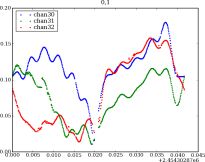
\includegraphics[scale=.23]{plot_uv1.png}
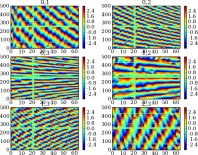
\includegraphics[scale=.23]{plot_uv2.jpg}\\
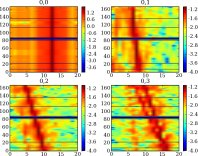
\includegraphics[scale=.23]{plot_uv3.jpg}
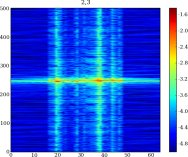
\includegraphics[scale=.23]{plot_uv4.jpg}\\
\caption{Outputs of plot\_uv.py from \S\ref{sec:plot_uv}. Upper-left is [1],
upper-right is [2], lower-left is [3], and lower-right is [4].}
\label{fig:plot_uv}
\end{center}
\end{figure}

The outputs of these commands are in Figure \ref{fig:plot_uv}.  Command [1]
uses -a to select baseline (0,1), -p to select polarization yy, -c to
select 3 individual channels (counting from 0), -t to select a range of
integrations, and -m lin to plot in linear mode.  The result
is a linear xy plot of the 3 channels vs. time for that baseline.

Command [2] selects all cross-correlations, polarization yy and uses
the phase plotting mode.  This time, axis coordinates have been switched
to physical coordinates, and -t is now interpreted as a range of Julian dates
for selecting integrations to plot.  The result is a time-frequency 
``waterfall plot'' for each cross-correlation, with color signifying phase.

Command [3] uses -a to select all baselines involving antenna 0.  The
-d flag takes the Fourier transform of the frequency axis to delay (or lag)
domain.  Since physical coordinates have been specified, -c selects the 
range of (lag) channels from -200 to 200 nanoseconds.  -x says to use
only every 3rd integration (handy for plotting many files with lots of data).
A logrithmic color scale is assumed since no -m option was specified. 
This produces a waterfall plot of lag vs. time.  The
cross-correlations reveal sources moving across the sky over time.

Finally, command [4] plots baseline (2,3) with -d for the delay transform,
and -f to take the Fourier transform of the time axis.  This yields an
image with the vertical axis being fringe rate, and the horizontal axis being
delay.  This is an image of the sky (in weird coordinates).  By decimating
the number of intergrations used with -x, we restrict the range of fringe
rates obtained, effectively acting as a range select in fringe-rate domain.
Axis coordinates again have been changed to physical coordinates.

\subsection{Under the Hood}

The best way to get under the hood is to read the source code.  There is really
only one thing I wanted to put in this section, and that is how to read and
write heterogenous header items.  Whereas variables are all of a single data
type, headers can potentially contain a series of values of different types.
To avoid having to drop down to C to write interfaces for these variables, I
have made available low-level routines to manipulate items: haccess(), hread(),
and hwrite().  The convention I have followed for implementing a heterogenous
header item is to list it in aipy.miriad.itemtable as having type `?'.  This
makes an attempt to read/write to this header item drop down to the UV method
\_rdhd\_special()/\_wrhd\_special().  Here you can add an entry of your own,
modeled after the ``freqs'' header item (or better yet, you can subclass
UV and add it to your subclass).

